    \documentclass[12pt,a4paper,fleqn]{article}
\usepackage{rmpackages}																% usual packages
\usepackage{rmtemplate}																% graphic charter
\usepackage{rmexocptce}																% for DS with cptce eval

%\cfoot{} 													% if no page number is needed
%\renewcommand\arraystretch{1.5}		% stretch table line height

\begin{document}
\normalem % makes emphasize italic again

\begin{header}
TP - Comme un parfum de lavande (1)
\end{header}

\begin{multicols}{2}
\begin{center}
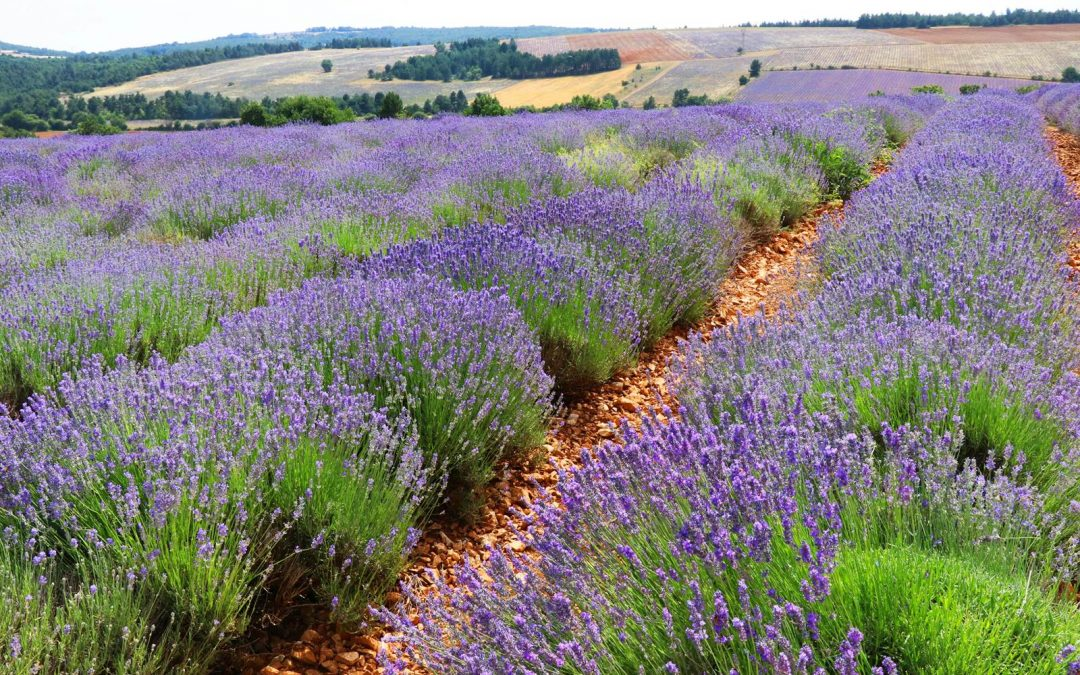
\includegraphics[width=\linewidth]{images/lavande.jpg}
\end{center}

L'\textbf{éthanoate de linalyle} est une espèce chimique utilisée notamment en parfumerie pour son odeur de lavande.
On la trouve en quantité importante dans l'huile essentielle de lavande ($\sim \qty{50}{\percent}$).

Cependant, il peut être avantageux de la synthétiser : \qty{1}{\litre} d'huile essentielle de lavande coûte environ 200 € alors que \qty{1}{\litre} d'éthanoate de linalyle synthétique ne coûte que 50 €.
Pour d'autres espèces, l'avantage peut être écologique, sanitaire, etc.
\end{multicols}

La réaction de synthèse est la suivante :
\[
\mathrm{ \underset{\text{linalol}}{C_{10}H_{18}O} + \underset{\text{anhydride acétique}}{C_4H_6O_3} \rightarrow \underset{\text{éthanoate de linalyle}}{C_{12}H_{20}O_2} + \underset{\text{acide éthanoïque}}{C_2H_4O_2}}
\]

\section*{Protocole expérimental}

\textcolor{red}{
\textbf{Pendant toutes les phases de manipulation, le port des lunettes de protection est obligatoire} !
\textbf{Le port des gants est indispensable pour certaines étapes.}
}

\paragraph{Synthèse de l'acétate de linalyle}
\begin{enumerate}
\item Introduire \qty{4}{mL} d'anhydride éthanoïque dans un ballon de \qty{250}{mL} \textbf{parfaitement sec}.
\item Ajouter \qty{2}{mL} de linalol et un grain de pierre ponce.
\item Placer le ballon dans le montage à reflux (Doc.~\ref{doc:reflux}).
\item Chauffer à reflux pendant \qty{30}{min}.
\end{enumerate}

\paragraph{Élimination de l'excès de réactif}
\begin{enumerate}[resume]
\item Arrêter le chauffage et laisser le ballon refroidir à l'air libre ($\sim\qty{15}{min}$).
\item Verser \qty{20}{mL} d'eau salée par le haut du réfrigérant.
\end{enumerate}

\paragraph{Extraction du produit}
\begin{enumerate}[resume]
\item Verser le contenu du ballon dans l'ampoule à décanter, sans la pierre ponce.
Rincer le ballon avec \qty{2}{mL} de cyclohexane (Doc.~\ref{doc:decantation}).
\item Agiter en dégazant régulièrement, laisser décanter puis \textbf{éliminer la phase aqueuse}.
\item \label{step:bicarbonate} Traiter la phase organique avec \qty{20}{mL} de solution d'hydrogénocarbonate de sodium.
\item Agiter en \textbf{dégazant très régulièrement}, laisser décanter puis éliminer la phase aqueuse.
\item Conserver la phase organique.
\end{enumerate}

\begin{multicols}{2}
\begin{doc}
\label{doc:reflux}
\textbf{Montage à reflux}

\begin{center}
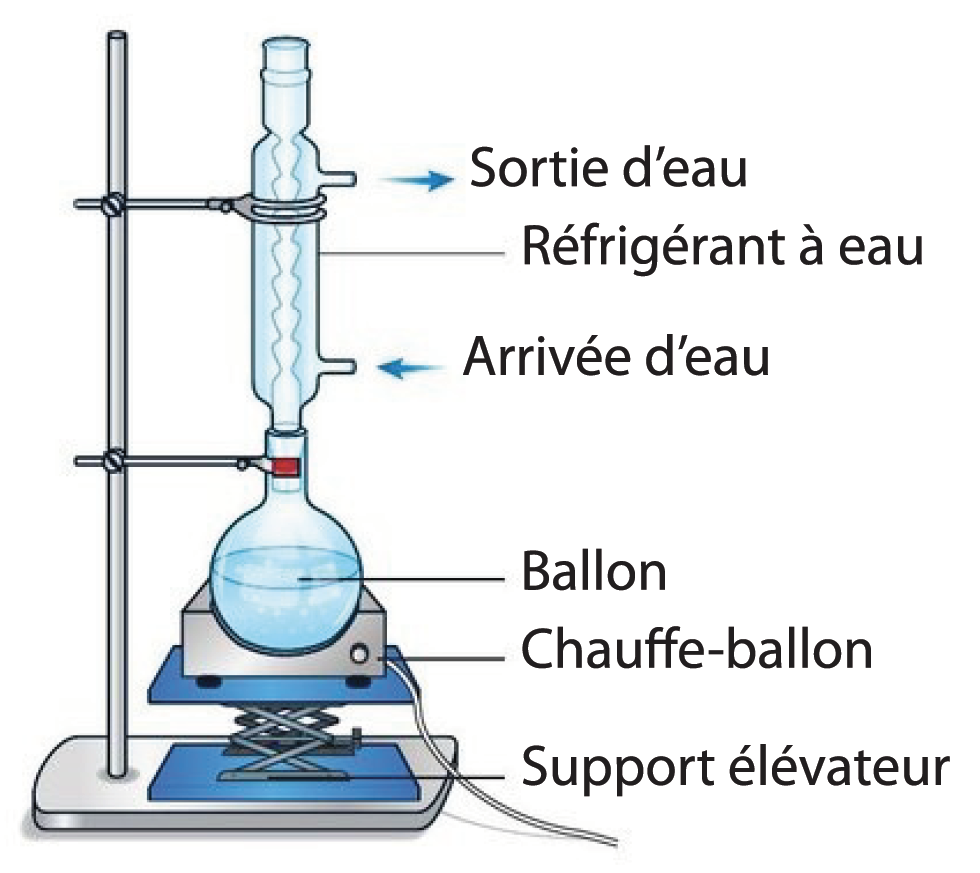
\includegraphics[height=180 pt]{images/reflux.png}
\end{center}
\end{doc}

\begin{doc}
\label{doc:decantation}
\textbf{Montage de décantation}

\begin{center}
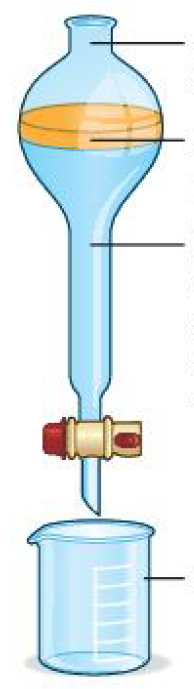
\includegraphics[height=180 pt]{images/decantation.png}
\hfill
\null
\end{center}
\end{doc}
\end{multicols}

\begin{doc}
\textbf{Données}
\begin{center}
\renewcommand\arraystretch{1.5}		% stretch table line height
\begin{tabular}{| >{\centering\arraybackslash}p{.15\linewidth} | *{4}{>{\centering\arraybackslash}p{.17\linewidth} |}}
\hline
 & \textbf{Linalol} & \textbf{Anhydride éthanoïque} & \textbf{Éthanoate de linalyle} & \textbf{Acide éthanoïque} \\
 \hline
\textbf{Densité} & \num{0.87} & \num{1.08} & \num{0.89} & \num{1.18} \\
\hline
$T_\mathrm{ébullition}$ (\unit{\degreeCelsius}) & \num{199} & \num{139.5} & \num{220} & \num{85} \\
\hline
\textbf{Solubilité dans l'eau} & Assez faible & Très élevée & Très faible & Très élevée \\
\hline
\end{tabular}
\end{center}
\end{doc}

\begin{doc}
\textbf{Pictogrammes de sécurité}

Les différents produits chimiques utilisés lors de cette synthèse présentent certains risques qu'il faut connaitre pour s'en protéger.

\begin{center}
\begin{tabular}[c]{|l| m{5.5cm} |}
\hline
\textbf{Linalol} & 
\includegraphics[trim=0 0 0 -75, height=40 pt]{images/pict_nocif.jpg} \\
\hline
\textbf{Anhydride éthanoïque} & 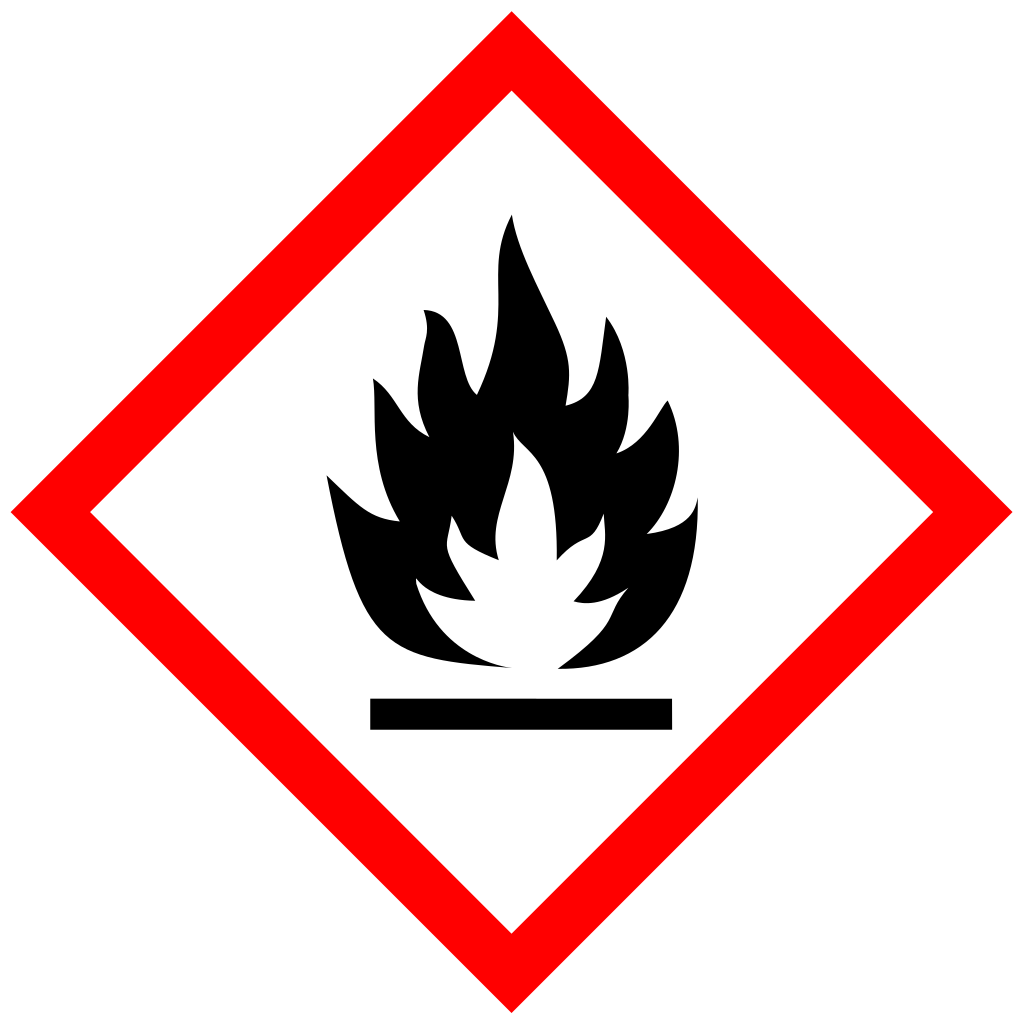
\includegraphics[trim=0 0 0 -75, height=40 pt]{images/pict_inflammable.png}  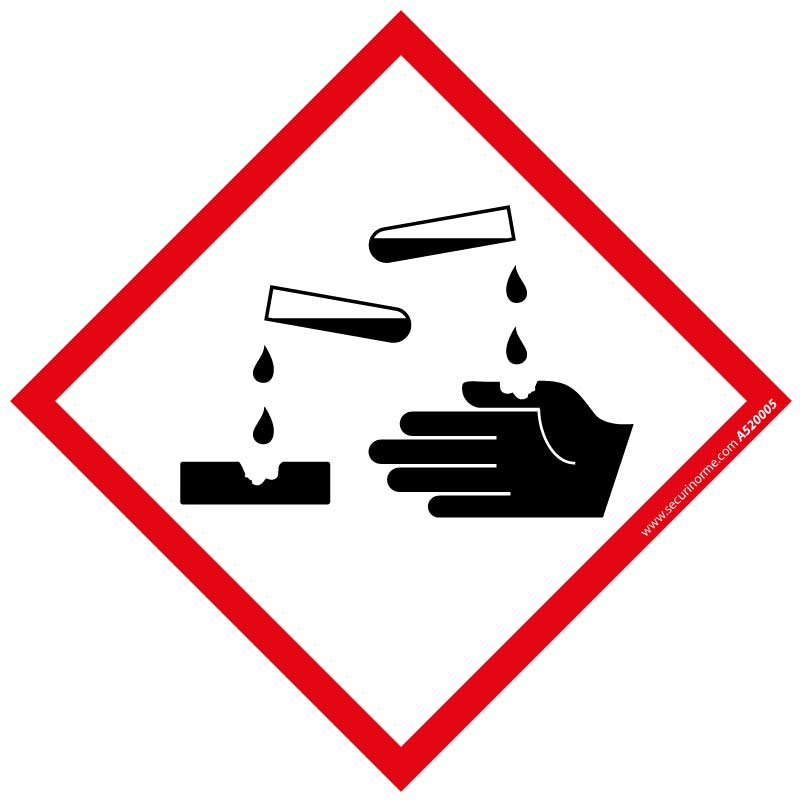
\includegraphics[trim=0 0 0 -75, height=40 pt]{images/pict_corrosif.jpg}   
\includegraphics[trim=0 0 0 -75, height=40 pt]{images/pict_nocif.jpg} \\
\hline
\textbf{Éthanoate de linalyle} & 
\includegraphics[trim=0 0 0 -75, height=40 pt]{images/pict_nocif.jpg} \\
\hline
\textbf{Cyclohexane} &  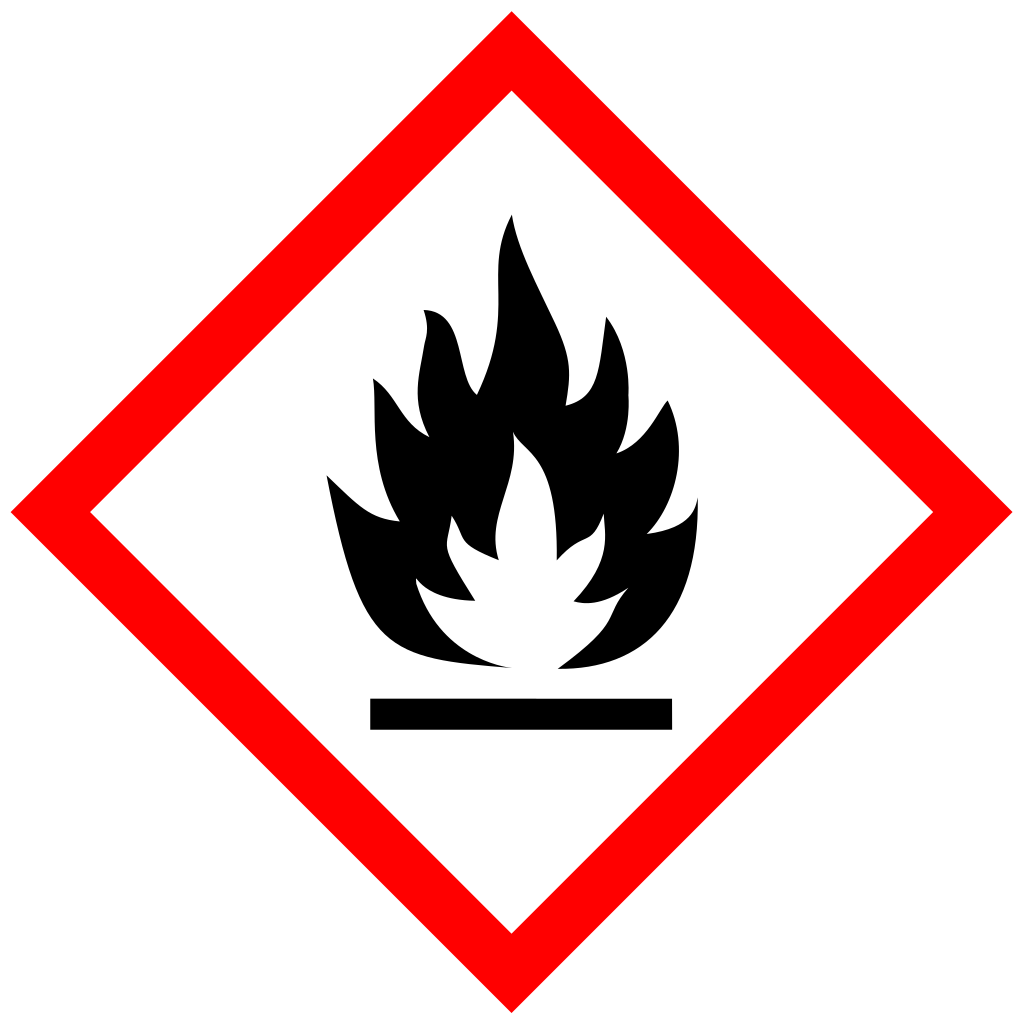
\includegraphics[trim=0 0 0 -75, height=40 pt]{images/pict_inflammable.png} 
\includegraphics[trim=0 0 0 -75, height=40 pt]{images/pict_cancer.jpg}

\includegraphics[trim=0 0 0 -75, height=40 pt]{images/pict_nocif.jpg} 
\includegraphics[trim=0 0 0 -75, height=40 pt]{images/pict_aquatique.jpg}  \\
\hline
\end{tabular}
\end{center}
\end{doc}

\section*{Questions}

\subsection*{Questions préliminaires}

\begin{enumerate}
\item \app

Identifier le produit chimique qui justifie particulièrement l'utilisation des gants.

\emph{Porter des gants n'est pas toujours une bonne idée : \href{https://youtu.be/QmCdrDLyNXQ?t=577}{https://youtu.be/QmCdrDLyNXQ?t=577}}.

\item \app

Identifier le produit chimique qui doit impérativement être utilisé sous hotte.

\item \anarai

Proposer une hypothèse sur la nécessité d'utiliser de la verrerie parfaitement sèche.
\end{enumerate}

\subsection*{La synthèse}

\begin{enumerate}[resume]
\item \anarai

À votre avis, pourquoi doit-on chauffer le mélange ?

\item \anarai

Proposer une hypothèse sur la nécessité du support élévateur dans le montage à reflux.
Et celle du réfrigérant à boule.
\end{enumerate}

\subsection*{Extraction}

\begin{enumerate}[resume]
\item \app{} \anarai{}

Écrire l'équation de la réaction qui se produit lors de l'étape~\ref{step:bicarbonate} et nommer le gaz formé.

\item \app{}

Légender le schéma du document~\ref{doc:decantation} en indiquant notamment où se trouve l'éthanoate de linalyle.
\end{enumerate}

\subsection*{Et ensuite ?}

\begin{enumerate}[resume]
\item \rco{} \anarai{}

Proposer un protocole permettant de vérifier que l'espèce synthétisée est présente dans l'huile essentielle de lavande.
\end{enumerate}

\end{document}